\documentclass[aps,prl,twocolumn,superscriptaddress,footinbib]{revtex4-1}
\usepackage[utf8]{inputenc}
\usepackage[colorlinks=true,linkcolor=cyan,citecolor=cyan,urlcolor=cyan]{hyperref}
\usepackage{bm,bbm,amssymb,amsmath}
\usepackage{graphicx}
\usepackage[dvipsnames]{xcolor}

\newcommand{\Msun}{\ensuremath{\,M_{\odot}}}
\newcommand{\apjl}{Astrophys. J. Lett.}

\newcommand{\FZU}{CEICO, FZU-Institute of Physics of the Czech Academy of Sciences,
Na Slovance 1999/2, 182 21 Prague 8, Czech Republic}
\newcommand{\CITA}{Canadian Institute for Theoretical Astrophysics, University of Toronto, Toronto, Ontario M5S 3H8, Canada}

\begin{document}

\title{Supplemental Material: Prospects for constraining twin stars with next-generation gravitational-wave detectors}

\author{Philippe Landry}
\affiliation{\CITA}
\author{Kabir Chakravarti}
\affiliation{\FZU}

\maketitle  

\paragraph{Twin-star equations of state.}\label{Sec_PT}

We provide further details about our choice of twin-star-supporting equations of state. The constant-sound-speed formulation~\cite{HanSteiner2019} we use to construct them consists of a low-density hadronic EOS, to which a constant-pressure first-order phase transition segment of strength $\Delta\rho$ is connected at onset density $\rho_t$. A high-density extension with constant sound speed is appended to the end of the phase transition segment. Within this formulation, we explore the region of the parameter space that satisfies existing constraints from neutron star observations.

In particular, if we suppose that the $\sim 1.4\Msun$ NSs observed in GW170817 and as PSR J0030+0451 are purely hadronic, then the low-density EOS must satisfy the approximate observational upper bounds $\Lambda_{1.4} \lesssim 580$~\cite{LVC_GW170817eos} and $R_{1.4} \lesssim 14$ km~\cite{MillerLamb2019}. (In fact, because the analysis in Ref.~\cite{LVC_GW170817eos} relies on EOS-insensitive relations that can't accommodate twin stars, we allow for some leeway in the first constraint.) If, instead, we suppose that those compact objects are hybrid stars, then the low-density portion of the EOS remains unconstrained. These considerations motivate the choice of SKI272 ($R_{1.4} \approx 13.5$ km, $\Lambda_{1.4} \approx 650$)~\cite{AgrawalShlomo2003} and SKI5 ($R_{1.4} \approx 14.5$ km, $\Lambda_{1.4} \approx 1000$)~\cite{ReinhardFlocard1995,BertulaniValencia2019} under the first and second scenarios, respectively. Both of these low-density EOSs have a symmetry energy slope $L \lesssim 140$, in keeping with the implications of the PREX-II experiment~\cite{ReedFattoyev2021}.

For the high-density extension, we select a causal EOS to increase the odds that stable twin stars will be supported. To interpolate between the high- and low-density regimes, we explore different first-order phase transition segments by selecting various combinations of onset density $\rho_t \in [1, 4]\rho_{\rm nuc}$ and strength $\Delta\rho \in (0,2]\rho_t$. For use in our study, we retain a representative subset of those EOSs that give rise to stable twin stars while simultaneously satisfying the approximate mass and radius constraints from electromagnetic observations of PSR J0740+6620: $M_{\rm TOV} \gtrsim 2.0\Msun$, $R_{2.0} \gtrsim 12$ km~\cite{MillerLamb2021}. The selected EOSs are plotted in Fig.~\ref{fig:Eos_plot}. Their phase transition parameters and associated NS observables are listed in Table~\ref{tab:eos}, while their $m$--$R$ and $m$--$\Lambda$ relations are plotted in the main text. The mass-radius relations are obtained by solving the Tolman-Oppenheimer-Volkoff equations~\cite{OppenheimerVolkoff1939,Tolman1939}. In each relation, there is a small range of masses for which a hybrid twin with a smaller radius and larger central density coexists alongside a hadronic star. Similar morphology is apparent in the mass-tidal deformability relations obtained by solving for a quadrupolar tidal perturbation~\cite{FlanaganHinderer2008,Hinderer2008,LandryPoisson2014}. Of particular relevance for our analysis is the unstable segment in the $m$--$\Lambda$ relation that connects the hadronic and hybrid branches at a mass scale corresponding to $\rho_t$.

\begin{figure}[tb]
    \centering
    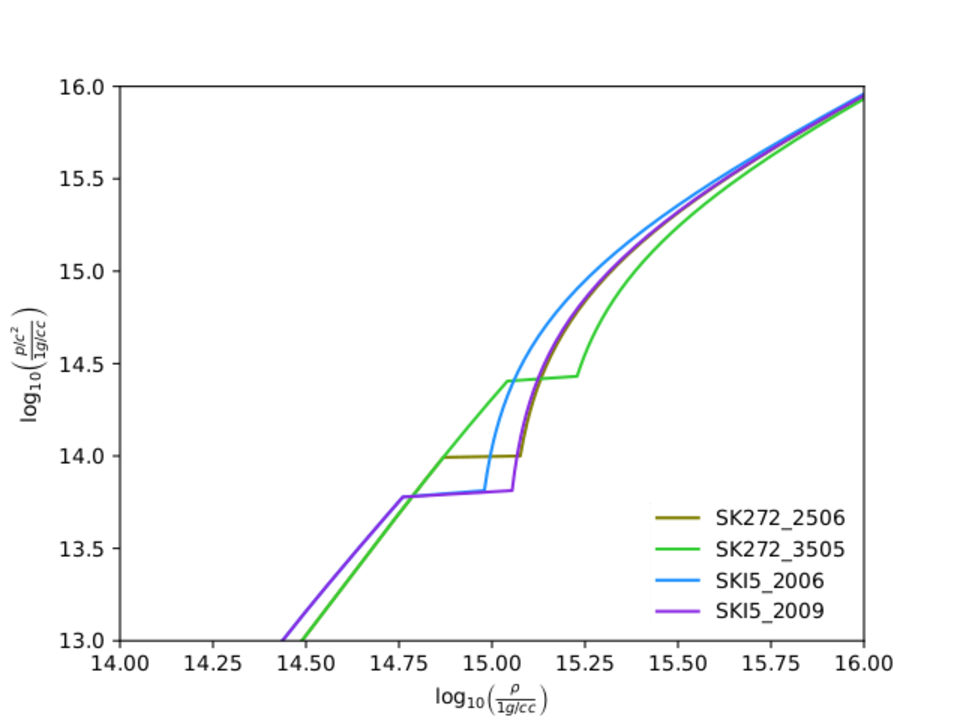
\includegraphics[width=0.9\columnwidth,trim={1 2 30 30},clip]{EoS.pdf}
    \caption{Twin-star--supporting equations of state used in this work. The discontinuities in baryon density at fixed pressure are first-order phase transitions of Maxwell type. The phase transitions occurring in these equations of state are strong enough to give rise to stable twin stars.}
    \label{fig:Eos_plot}
\end{figure}

\begin{table*}[tb]
    \centering
    \begin{tabular}{lcccccccc}
    \hline \hline
    EOS & $\rho_t\;[\rho_{\rm nuc}]$ & $\Delta\rho\;[\rho_{t}]$ & $\Delta M_{t}\;[M_{\odot}]$ & $M_{\rm TOV}\;[M_{\odot}]$ & $R_{1.4}\;$[km] & $\Lambda_{1.4}$ & $M_t\;[M_{\odot}]$ & $\Delta\Lambda$ \\ \hline    
     SKI5\_2006 & 2.0 & 0.6 & 0.01 & 2.28 & 13.5 & 520  & 1.36 & 340 \\
     SKI5\_2009 & 2.0 & 0.9 & 0.07 & 2.08 & 12.2 & 240 & 1.32 & 940 \\
     SK272\_2506 & 2.5 & 0.6 & 0.01 & 2.08 & 13.5 & 650 & 1.45 & 80 \\ 
     SK272\_3505 & 3.5 & 0.5 & 0.03 & 1.94 & 13.5 & 650 & 1.91 & 40 \\ \hline \hline
    \end{tabular}
    \caption{Twin-star-supporting equations of state used in this study. The parameters $\rho_t$ and $\Delta\rho$ specifying the onset density and strength of the first order phase transition are listed. The mass range $\Delta M_t$ over which twins are supported, the maximum mass $M_{\rm TOV}$, and the canonical radius $R_{1.4}$ and tidal deformability $\Lambda_{1.4}$ for the corresponding sequence of neutron stars are also given. Additionally, we list the twin-star mass scale $M_t$ and tidal deformability difference $\Delta\Lambda$ that we seek to recover via hierarchical inference. The equation of state's name indicates the low-density hadronic model upon which it is based.}
    \label{tab:eos}
\end{table*}

\paragraph{Morphology of the tidal deformability distribution.}

In the main analysis, we argue that an EOS's support for twin stars translates into a disjoint two-dimensional distribution of binary tidal deformability

\begin{equation}
    \tilde{\Lambda} = \frac{16}{13} \frac{(1+12q) \Lambda_1 + (q+12)q^4\Lambda_2}{(1+q)^5}
\end{equation}
vs chirp mass

\begin{equation}
    \mathcal{M} = \frac{(m_1 m_2)^{3/5}}{(m_1+m_2)^{1/5}} ,
\end{equation}
whereas the equivalent distribution is contiguous for an EOS without a disconnected hybrid star branch.
The gaps in the distribution originate directly from the unstable segment of the $m$--$\Lambda$ relation that connects the hadronic and hybrid branches for twin-star-supporting EOSs.
They correspond to strong first-order phase transitions in the EOS, where the baryon density jumps discontinuously at fixed pressure, as shown in Fig.~\ref{fig:Eos_plot}.
The gaps in the $\tilde{\Lambda}$ vs $\mathcal{M}$ distribution occur where, along lines of constant mass ratio $q = m_2/m_1$, one component mass lies on the unstable segment.
This is illustrated in Fig.~\ref{fig:lambdapop2}, which breaks down the distribution along lines of fixed mass ratio.
The upper (respectively, lower) gap in the distribution for SKI5\_2009 corresponds to $m_2$ ($m_1$) lying on the unstable segment. Note how a similar breakdown of the distribution for the purely hadronic SKI5 EOS does not evince any gaps.

Figure~\ref{fig:lambdapop2} also shows the same distribution for SK272\_3505 and its purely hadronic counterpart, SK272. In this case, due to its very small twin-star mass range $\Delta M_t$ and tidal deformability difference $\Delta\Lambda$ between twins, the gaps in the distribution for SK272\_3505 are barely visible at scale. However, along lines of constant mass ratio, one can see the distribution is broken into distinct segments. Again, this contrasts with the continuous distribution for SK272.

\begin{figure}[b]
    \begin{tabular}{c}
      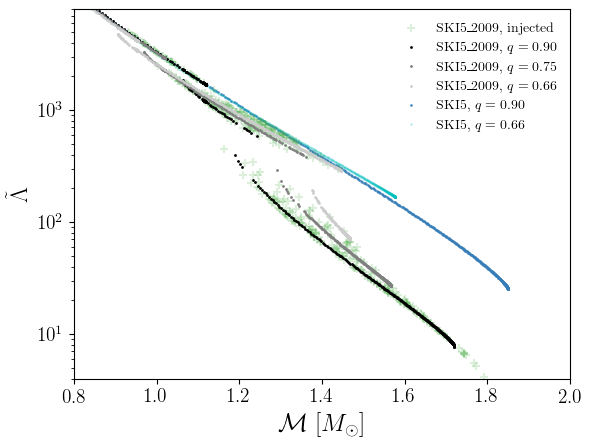
\includegraphics[width=0.9\columnwidth]{SKI52009_sm.png} \\
      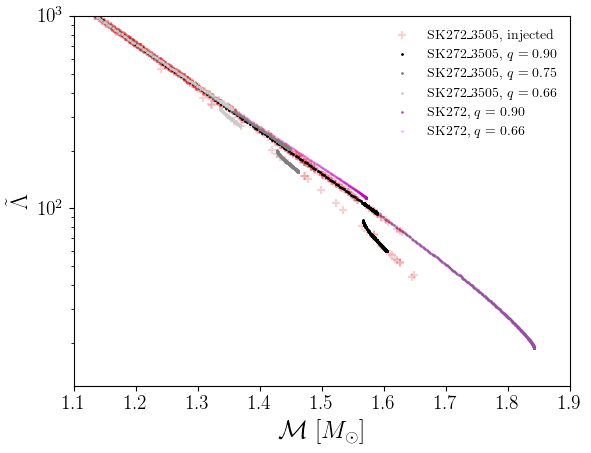
\includegraphics[width=0.9\columnwidth]{SK2723505_sm.png}
    \end{tabular}
    \caption{The joint binary tidal deformability and chirp mass distribution probed by one month of XG observations for selected equations of state studied in this work. The distribution is broken down according to mass ratio, showing how the gaps that indicate the presence of twin stars arise. A uniform neutron star mass distribution is assumed.}
    \label{fig:lambdapop2}
\end{figure}

\paragraph{Simulated binary neutron star population.}

We supply additional information about the procedure by which we generate mock detected populations of binary neutron star mergers. Our NS mass distribution is chosen to be uniform for $m \in [1\Msun,M_{\rm TOV}]$ based on studies of the GW population to date~\cite{LandryRead2021,LVK_O3bPop}. 
We assume that both components of a NS binary are drawn from this common mass distribution, and that they pair randomly.
We distribute the sources isotropically on the sky and according to a Madau-Dickinson star formation rate~\cite{MadauDickinson2014} in redshift. 
The local, astrophysical BNS merger rate of 440 Gpc$^{-3}$ y$^{-1}$ that we adopt corresponds to the 90\% confidence upper bound from Ref.~\cite{LVK_O3bPop}'s PowerLaw+Dip+Break model.

We calculate optimal signal-to-noise ratios for the simulated mergers with respect to the HLV, A+ and XG networks described in the main text. For the HLV and A+ networks, we simulate mergers within their projected luminosity distance ranges of 190 Mpc and 330 Mpc, respectively, for BNSs~\cite{AbbottAbbott2018_ObservingScenarios}. 
For the XG network, whose BNS range will extend to cosmological distances~\cite{EvansAdhikari2021,BorhanianSathyaprakash2022}, we simulate only the nearby mergers ($z \lesssim 0.5$) that contribute the loudest events. Our SNR calculation is carried out with \texttt{bilby}~\cite{AshtonHubner2019}, using the \texttt{IMRPhenomPv2\_NRTidal} waveform model~\cite{DietrichKhan2019}, a minimum frequency of 10 Hz (40 Hz for HLV), and a network SNR threshold of 12 for detection.

For each detected event, we simulate the likelihoods in chirp mass $\mathcal{M}$, mass ratio $q$ and binary tidal deformability $\tilde{\Lambda}$ as independent Gaussians, scaling their standard deviations with the event's SNR in inverse proportion to GW170817's~\cite{FarrBerry2016}. We mock up the effect of the detector noise realization by adding Gaussian noise that shifts the median of the likelihood within one standard deviation.

\begin{figure*}
    \begin{tabular}{cc}
      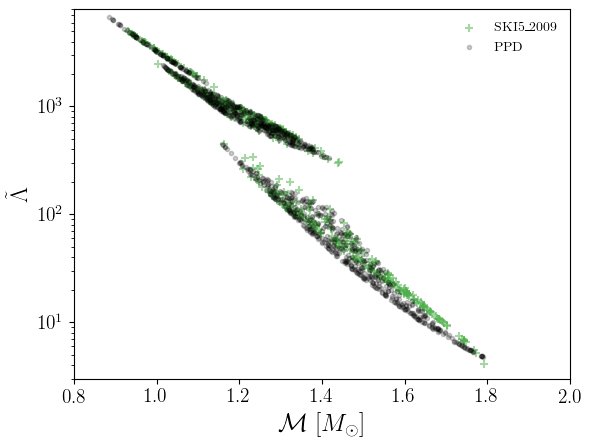
\includegraphics[width=0.9\columnwidth]{SKI52009_ppd.png} &
      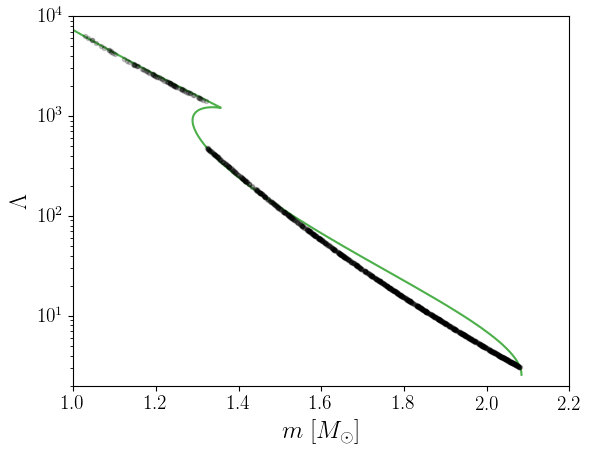
\includegraphics[width=0.9\columnwidth]{SKI52009_ppd2.png} \\
      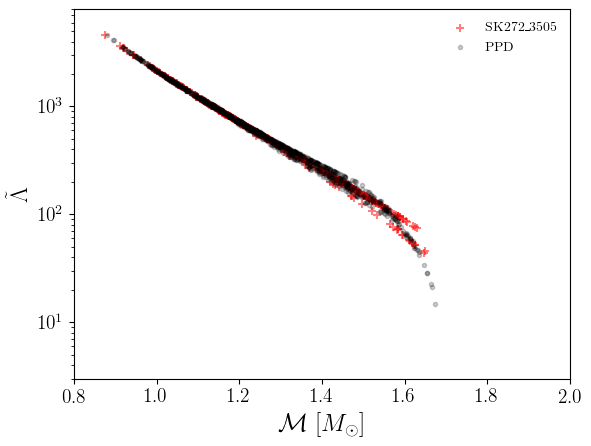
\includegraphics[width=0.9\columnwidth]{SK2723505_ppd.png} &
      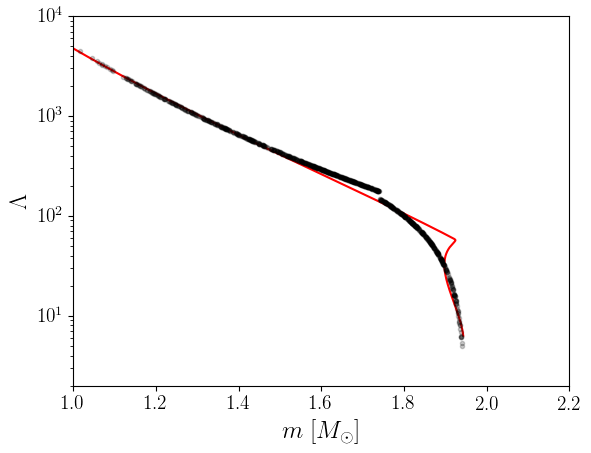
\includegraphics[width=0.9\columnwidth]{SK2723505_ppd2.png}
    \end{tabular}
    \caption{Posterior predictive checks for selected twin-star-supporting equations of state. We compare the posterior predictive distribution for the binary tidal deformability vs chirp mass distribution (left) and the mass--tidal deformability relation (right) to the injected values. The posterior predictive distribution is constructed from the approximate mode of the recovered three-dimensional posterior in $\Delta\Lambda$, $M_t$ and $k$.}
    \label{fig:ppd}
\end{figure*}

\paragraph{Posterior predictive checks.}

To support our main results, we perform posterior predictive checks and examine how constraints on the twin-star parameters evolve with the number of BNS detections. For each injected EOS, we extract the approximate maximum-likelihood parameters ($\Delta\Lambda$,$M_t$,$k$) from the population-averaged posterior after one month of XG observations. We use these parameters to reconstruct the best-fit $m$--$\Lambda$ relation according to the parameterization introduced in the main text. We then sample a uniform BNS population and reconstruct the predicted distribution of binary tidal deformability vs chirp mass for the population. Figure~\ref{fig:ppd} compares these predictions for the $m$--$\Lambda$ relation and the $\tilde{\Lambda}$ vs $\mathcal{M}$ distribution to their true values for two selected EOSs, SKI5\_2009 and SK272\_3505. These are respectively the best- and worst-recovered examples.

For SKI5\_2009, we observe that the predicted distributions are close, but not perfect, matches to the injected ones. The main discrepancy occurs at large masses, where the model's fixed power-law slope does not allow for the flexibility required to track the actual $m$ vs $\Lambda$ trend. This is essentially a deliberate tradeoff in the model, which prizes simplicity over fidelity. Similarly, by construction, the model does not track the $m$--$\Lambda$ relation right through the unstable segment connecting the hadronic and hybrid branches. However, our simplified treatment of this juncture manifestly reproduces the right $\tilde{\Lambda}$ vs $\mathcal{M}$ morphology and accurately locates the discontinuity in the $m$--$\Lambda$ relation.

For SK272\_3505, which has a much higher phase transition onset density and much smaller $\Delta M_t$ and $\Delta\Lambda$, the model clearly struggles to match both the location and extent of the hybrid branch. The mode of the posterior, upon which the illustrated posterior predictive check is based, favors a good fit to the latter at the expense of the former. However, as this EOS is the one with the largest uncertainties \textit{a posteriori}, the posterior encompasses other parameter combinations that recover the twin star mass scale more accurately.

This can be seen in the evolution of the twin star parameter uncertainties as a function of the number of $z < 0.5$ BNS detections. In Fig.~\ref{fig:params}, we show the posterior 90\% confidence intervals on $\Delta\Lambda$ and $M_t$ for the different observing scenarios we consider. The parameters are recovered accurately for all of the EOSs, except for a slight underestimate of $M_t$ in the case of SK272\_3505, which is related to the mismatch in the posterior predictive check. The precision in the parameter measurements increases significantly when passing from the A+ to the XG detector network.

\begin{figure*}
    \begin{tabular}{cc}
      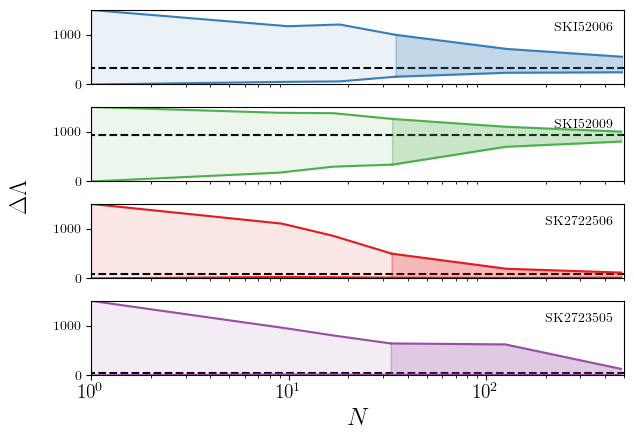
\includegraphics[width=0.45\textwidth]{DeltaL_convergence.png}   & 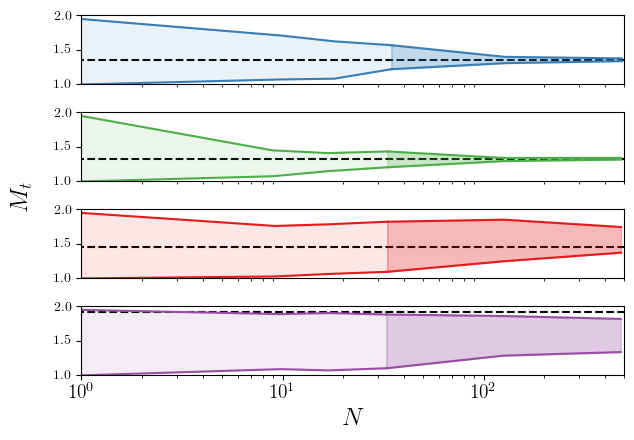
\includegraphics[width=0.45\textwidth]{Mt_convergence.png}
    \end{tabular}
    \caption{Constraints on the tidal deformability difference between twins and the twin-star mass scale as a function of the number of binary neutron star mergers detected within a redshift $z < 0.5$. We show the evolution of the 90\% confidence contours. The era of A+ (respectively, XG) observations is shown with lighter (darker) shading. We average over 10 population realizations to mitigate fluctuations in statistical uncertainties.}
    \label{fig:params}
\end{figure*}

\paragraph{Robustness of our conclusions.}

Our precise forecasts for A+ and XG parameter constraints obviously depend on the specific EOSs chosen for study. While our analysis is not an exhaustive exploration of the parameter space for twin stars, we consider a variety EOSs with first-order phase transitions of different onset densities and strengths. Besides the choice of EOS, our forecasts also depend in principle on assumptions about the NS mass distribution and the relative abundance of hadronic vs hybrid twins in the detected population. We revisit some of these choices and demonstrate that reasonable alternative assumptions do not significantly alter the recovery of the twin-star parameters.

\begin{enumerate}
    \item \textit{Effect of the population realization:} The main results average over 10 realizations of the BNS population. In Fig.~\ref{fig:results_indiv}, we investigate how much the parameter constraints vary with the population realization: we show the two-dimensional posterior 90\% confidence contours on $\Delta\Lambda$ and $M_t$ for SKI5\_2009 for five population realizations after two years of A+ observations and one month of XG observations---these are the best-case A+ and XG observing scenarios, respectively. One can see that statistical fluctuations due to the population realization can significantly impact the A+ contours; however, as the detector network improves and the number of observations increases, this variability becomes less significant.
    
    \item \textit{Effect of the branching ratio:} Our main results assume that NSs with masses in the twin star range lie with equal probability on the hadronic or hybrid branch of the $m$--$\Lambda$ relation. Here we make an alternative choice and show that the twin-star parameter constraints are largely unchanged in our best-case scenario.  We assume that twin stars are distributed uniformly in central density, such that the probability for an arbitrary twin star to lie on the hadronic vs the hybrid branch is proportional to the ratio of density ranges supported by each twin-star branch. For instance, if hadronic twins span a central density range of $0.3\,\rho_{\rm nuc}$, and hybrid twins span only $0.1\,\rho_{\rm nuc}$, there should be three times as many hadronic twins as hybrid ones. Repeating the analysis for the SKI5\_2009 EOS under these conditions, we obtain Fig.~\ref{fig:bimod_results}'s population-averaged posterior on the parameters $\Delta\Lambda$ and $M_t$. As was the case under the original branching ratio assumption, twin stars are definitively identified in the population after one week of XG observations.

    \item \textit{Effect of the mass distribution:} In the main analysis, we adopted a uniform mass distribution for the BNS population.
    We now revisit that assumption and demonstrate that our conclusions are unchanged if we instead use the bimodal NS mass distribution from Ref.~\cite{FarrChatziioannou2020}, inspired by observations of Galactic pulsars. We continue to assume that NSs pair randomly into binaries.
    When we repeat the analysis with this alternative population model, we obtain the twin-star parameter constraints shown in Fig.~\ref{fig:bimod_results}.
    The results are averaged over 10 population realizations.
    We obtain qualitatively similar constraints as with the uniform NS mass distribution: one month of XG observations can identify the presence of twin stars in the SKI5\_2009 and SKI5\_2006 scenarios, while $\Delta\Lambda \gtrsim 100$ is ruled out in the other four scenarios.
    
\end{enumerate}

\begin{figure}[t]
      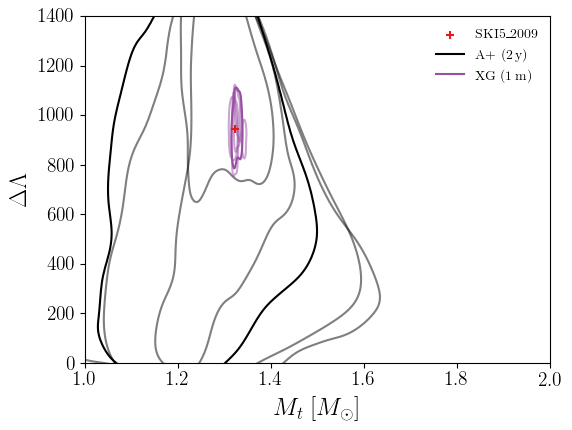
\includegraphics[width=0.9\columnwidth]{SKI52009_pops.png}
    \caption{Posteriors on twin-star parameters of the mass-tidal deformability relation for the SKI5\_2009 equation of state. The 90\% credible region of the posterior is shown for the best-case A+ and XG observing scenarios we consider. We show how the credible regions differ across several different population realizations (faint traces) compared to the population averages (solid lines). Note how the variation due to the population realization diminishes as more observations are accumulated.}
    \label{fig:results_indiv}
\end{figure}

\begin{figure}[t]
    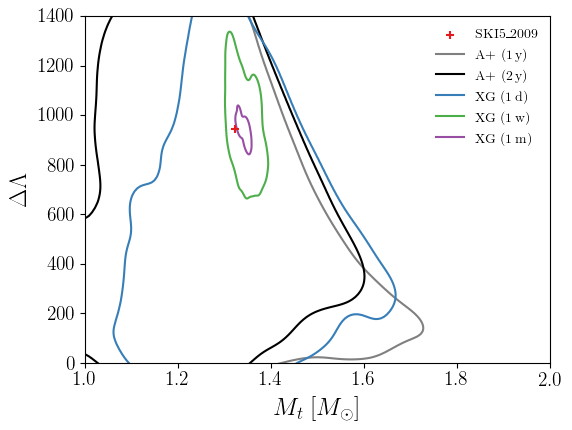
\includegraphics[width=0.9\columnwidth]{SKI52009_br.png}
    \caption{Posteriors on twin-star parameters of the mass-tidal deformability relation for the SKI5\_2009 equation of state, under a different assumption about the hadronic vs hybrid branching ratio for twin stars. The 90\% credible region of the posterior, averaged over 10 population realizations, is shown for various observing scenarios. Note the qualitative similarity with the equivalent figure in the main text.}
    \label{fig:branch_results}
\end{figure}

\begin{figure*}
    \centering
    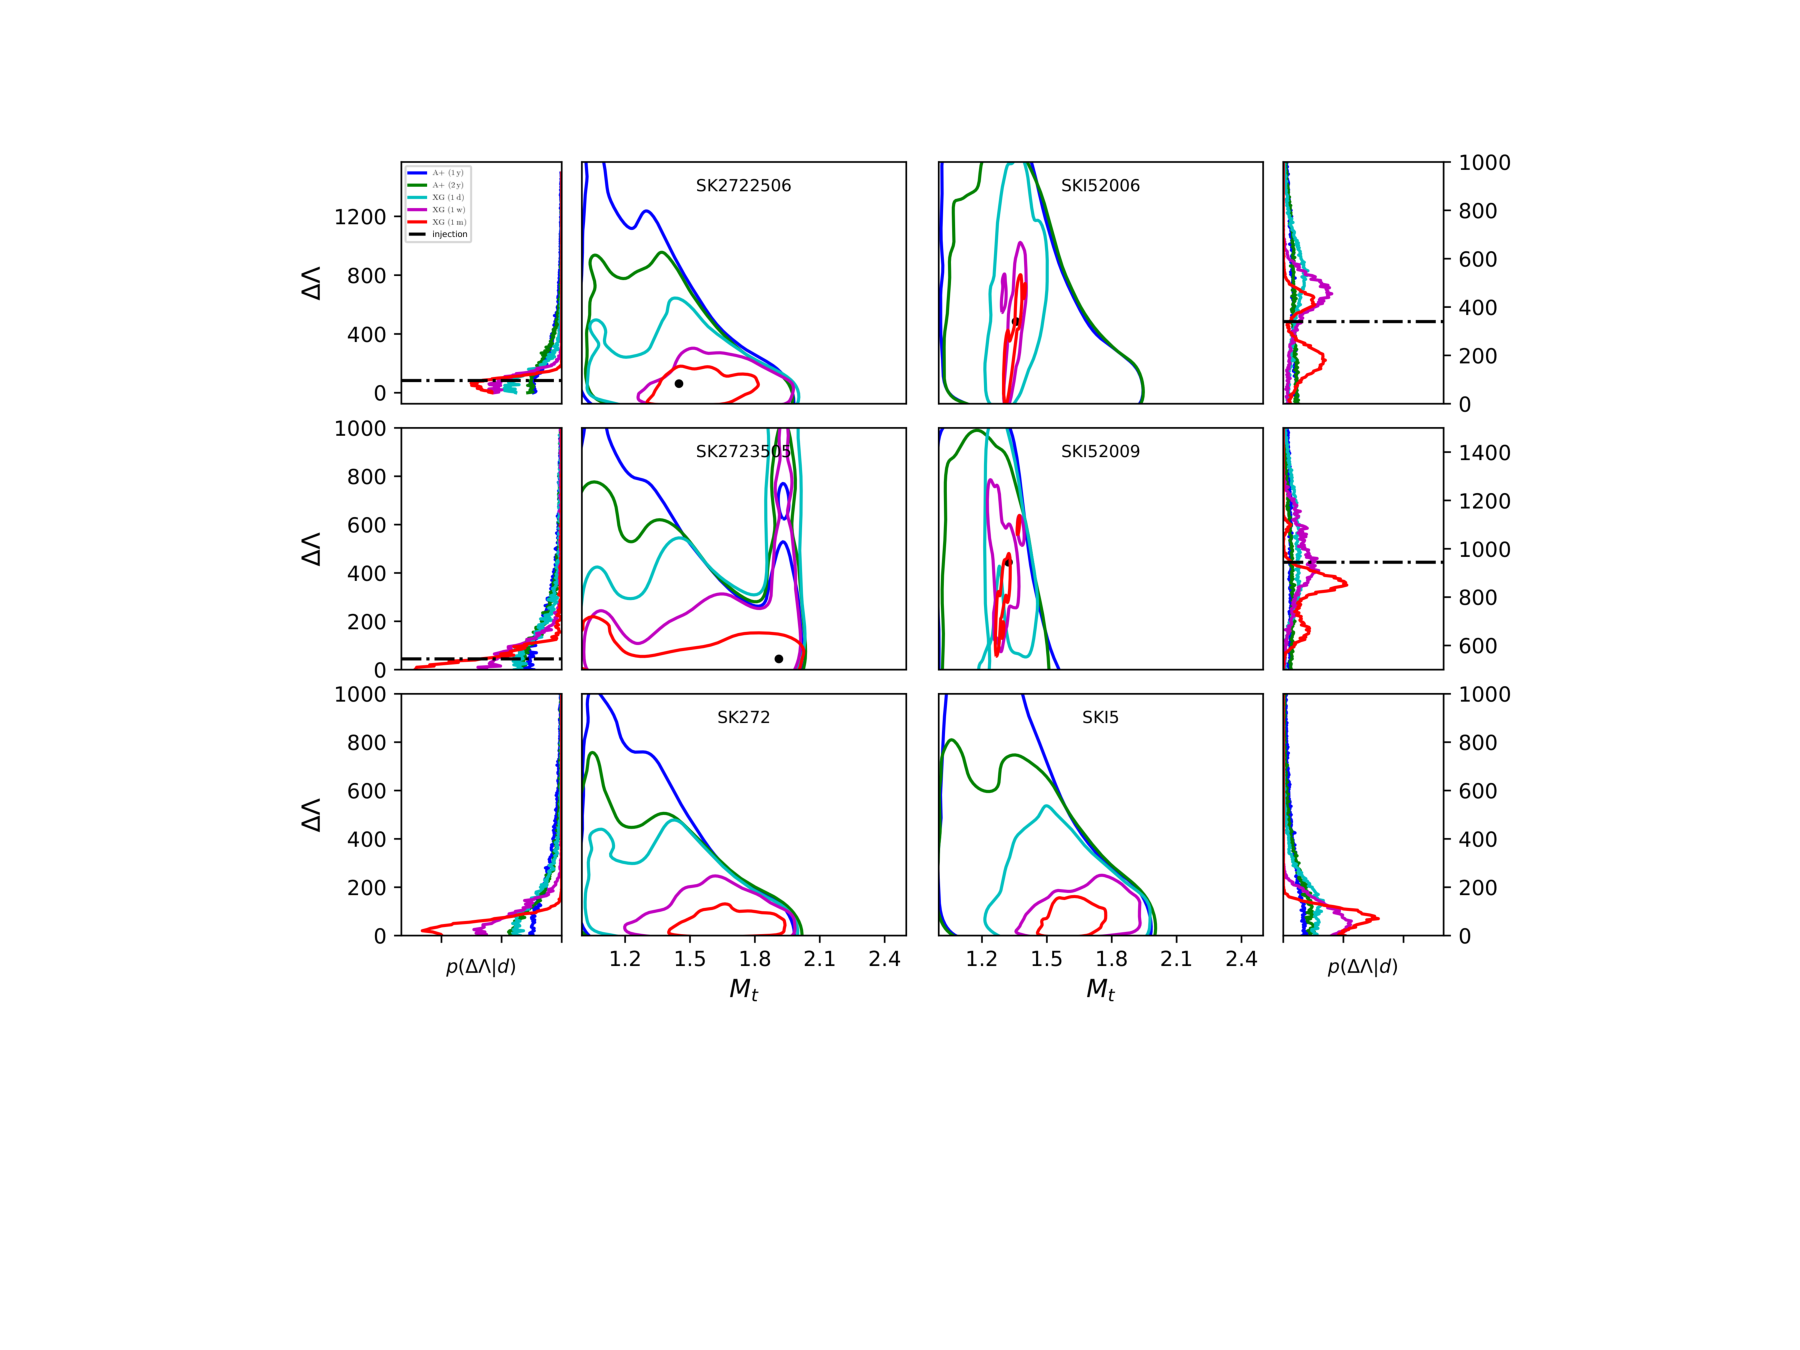
\includegraphics[width=0.9\textwidth,trim={145 160 130 70},clip]{bimod-moneyplot.pdf}
    \caption{Posteriors on twin-star parameters of the mass-tidal deformability relation for different equations of state, under the assumption of a bimodal neutron star mass distribution. The 90\% credible region of the posterior, averaged over 10 population realizations, is shown for various observing scenarios. Note the qualitative similarity with the equivalent figure in the main text.}
    \label{fig:bimod_results}
\end{figure*}

\bibliographystyle{apsrev4-1}
\bibliography{references}

\end{document}
